\documentclass[a4paper,12pt]{report}
\setlength{\textwidth}{6.25in} % original 6.25
\setlength{\textheight}{8in}
\renewcommand{\baselinestretch}{1.3}
\oddsidemargin 20pt    %  Left margin on odd-numbered pages.
\evensidemargin 20pt   %  Note that \oddsidemargin = \evensidemargin
\topmargin 0pt
\usepackage {graphicx}
\usepackage{fancyhdr}
\usepackage{textcomp}
\usepackage{gensymb}
\usepackage{multirow}
\usepackage{makecell}
\usepackage{adjustbox}
\usepackage{natbib}
\usepackage{float}
\usepackage{amsmath}

\pagestyle{fancy}

\begin{document}
\begin{titlepage}
    \begin{center}
        \vspace*{0.5in}
        
        \Huge
        \textbf{Galaxy Morphology Classification}
        \vspace{0.2in}
        
        \normalsize
        \textbf{Shreyas Kalvankar}
        
        \vspace{0.5cm}
        Guided by - \\
        Prof. Seema Gondhalekar
        
        \vspace*{1.25in}
        
        
        \huge
        Seminar Report
        
        \vspace*{1.25in}
        \footnotesize
        \begin{center}
             
\includegraphics[width=0.5\textwidth]{figures/Logo.png}
        \end{center}
        K. K. Institute of Engineering Education and Research\\
        Department of Computer Engineering\\
        A.Y. 2019-20 Sem II
    \end{center}
\end{titlepage}

\chapter*{Acknowledgements\markboth{Acknowledgements}{Acknowledgements}}

\thispagestyle{empty}

\hspace*{0.5 in}First and foremost, I would like to thank my seminar guide, \textbf{Prof. S. K. Gondhalekar}, for her guidance and support. I will forever remain grateful for the constant support and guidance extended by my guide, in making this seminar report. Through our many discussions, she helped me to form and solidify ideas.\\
\hspace*{0.5 in} With a deep sense of gratitude, I wish to express my sincere thanks to, \textbf{Prof. Dr. S. S. Sane} for his immense help in planning and executing the works in time. My grateful thanks to the departmental staff members for their support.\\
\hspace*{0.5 in}I would also like to thank my wonderful colleagues and friends for listening my ideas, asking questions  and providing feedback and suggestions for improving my ideas.

\vspace*{1.3 in}
\hspace*{4 in}  Mr. Shreyas Kalvankar

\chapter*{Abstract\markboth{Abstract}{Abstract}}
\thispagestyle{empty}
\hspace*{0.5 in}Galaxy morphology classification is of immense importance to study the origin of the galaxy to analyze the space surrounding the galaxy. A number of features such as the age, existence of gravitational anomalies, position of the galaxy in the supercluster, etc can be extracted by the shape and size of a particular galaxy. The count of the shape of galaxies can be helpful in determining the true nature of the growth of galaxies. The belief that the Hubble Tuning fork diagram shows the evolution of galaxies from simple to complex \citep{hubble1926extragalactic} can be tested in accordance with the research.  
The paper \cite{dai2018galaxy} presented aims to propose a variant of residual network (ResNets), along with other popular Convolutional Neural Networks, for Galaxy Morphology Classification. It has been applied over a large set of training images from the Galaxy Zoo 2 dataset to classify the galaxies into five shapes namely spiral, edge-on, cigar-shaped smooth, in-between smooth, completely round smooth. The paper has provided different metrics such as accuracy, precision, recall values, etc to prove the performance to be better than the state of the art networks such as AlexNet, VGG, Inception and ResNets. The classification accuracy of the model on the testing set is given to be 95.2803\% with accuracy of each class separately defined. The model can be applied to large-scale galaxy classification in forthcoming surveys.

\newpage
\thispagestyle{empty}
\tableofcontents
\thispagestyle{empty}
\listoffigures
\thispagestyle{empty}
\listoftables
\thispagestyle{empty}
\newpage	
\pagenumbering{arabic}
\lhead{\bfseries Galaxy Morphology Classification}
\chapter{Introduction}
\hspace*{0.5 in}Studying galaxies and classifying them into different classes is a problem not of ephemeral nature. Physicists have been trying to identify and segregate galaxies into individual groups and study their discrete traits to understand the formation of these galaxies and relating the physics that creates them. Morphology is determined by the physical characteristics and the orbital structure of the galaxies. The shape of the galaxy potentials determines which orbital families are present. Stars moving in the specific parts of the space phase generate morphological features such as bars, rings, peanut bulges, pseudo-bulges, etc. Gases pile up close to orbital resonances producing regions of star formation. By looking at the morphology of a particular galaxy, we can learn about the history of star formation and secular evolution of galaxies. The stability of such features tells us about distribution of mass throughout the galaxy both dark and luminous.
\section{History of Galaxy Morphology and classes}
\hspace*{0.5 in}The first classification scheme of galaxy morphology was proposed by Edwin Hubble, 1926. The classification diagram was termed "The Hubble Sequence" that used visual inspection by classifying fewer than 400 galaxies. The Hubble Sequence (also called "Hubble Tuning Fork") classified the galaxies into three basic classes: spiral, elliptical, irregular \citep{hubble1926extragalactic}.\\
\begin{figure}[t]
\begin{center}
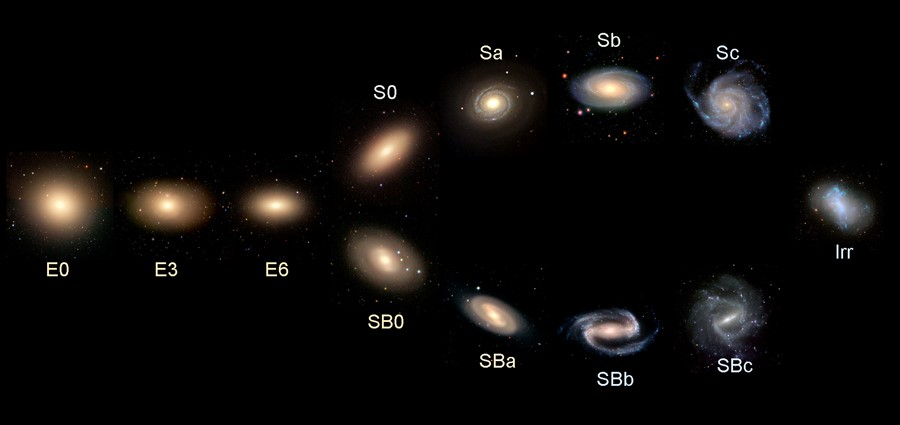
\includegraphics[width=\textwidth, height=.5\textheight]{figures/HubbleTuningFork2.jpg}
\caption{The Hubble Sequence}
\label{HubbleTuningFork}
\end{center}
\end{figure}
\hspace*{0.5 in}One of the major challenges in studying the morphologies is the techniques used for measurements. Before the computerized era of astrophysics, the technique of visual inspection and classification has been used by experts for several decades \citep{hubble1926extragalactic,Vaucouleurs,Edmondson464,VanDenBergh}.\\
\hspace*{0.5 in}The computerized era of astrophysics has revolutionized galaxy morphology classification. Both parametrized \citep{1968adga.book.....S,Cohen} and non-parametrized approaches have been used along with combined approaches \citep{2003ApJS..147....1C,2004AJ....128..163L} to reduce each galaxy to one number. This approach enables the processing of large scale images from different sky surveys \citep{Djorgovski_2013} and also helps provide a uniform quantitative set of parameters.\\
\hspace*{0.5 in}The previous methods of classification like visual inspection, however effective, were not able to cope with the sheer volume of data provided by the modern sky surveys such as the SDSS (Sloan Digital Sky Survey). This called for a better classification methodology which could process a huge amount of data with much more efficiency.

\section{Space surveys and galaxy classification}
\hspace*{0.5 in}The previous methods of classification like visual inspection, however effective, were not able to cope with the sheer volume of data provided by the modern sky surveys such as the SDSS (Sloan Digital Sky Survey). This called for a better classification methodology which could process a huge amount of data with much more efficiency. Some experts have performed extensive work in the detailed classification of the subset of the SDSS images.\\
\hspace*{0.5 in}The The Galaxy Zoo 1 project obtained more than 40,000,000 classifications made by approx. 100,000 participants. In the next phase \cite{Lintott_2010} included the data release of nearly 900,000 galaxies. The paper presented the measures of classification accuracy and bias. The data from \cite{2008MNRAS.389.1179L} was substantially reduced by comparing with the professional catalogues. Data reduction was performed and no prominent changes were observed after cross-checking. The samples with 80\% agreement among the users were labelled as 'clean' and with 95\% agreement among the users were called 'superclean' samples. The accuracy of the samples that were created by collecting data clicks and forming them into a scientific catalogue was very close to the actual morophology feature that the galaxy possessed.\\
\hspace*{0.5 in}The Galaxy Zoo 2 project was launched later and \cite{Willett_2013} produced the data release of nearly 16 million morphological classification with 304,122 galaxies, drawn from the SDSS. While the original Galaxy Zoo project identified galaxies as early-types, late-types or mergers, GZ2 measures finer morphological features \cite{Willett_2013}. This data release allowed a complete study of the finer morphological features and the co-relation of these features with properties of the galaxies i.e. mass, stellar and gas content, environment.As mentioned in the paper, although proxies such as spectral features, surface brightness profile, have been used extensively, they cannot be a replacement for for full morphological classification as pointed out by \cite{Lintott_2010}.This data has been used in studies of galaxy formation and evolution \citep{Land_et_all_2008,Schawinski,Willett_2015}.\\
\hspace*{0.5 in}The third phase in the crowd sourced visual classification was brought forward by \cite{Willet2016HST}. The new Galaxy Zoo : HST legacy imaging presented the data release of the Galaxy Zoo: Hubble (GZH). The GZH mainly focused on drawing surveys conducted by the Hubble Space Telescope to view the earlier epochs of galaxy formation. It's data contained measurements of disc- and bulge-dominated galaxies, spiral disc structure details that relate to Hubble type, identification of bars and measurements of clump identification. \cite{Willet2016HST} also suggests new methods of calibrating galaxies at different luminosities and at different redshifts by artificially redshfiting the galaxies and using them as a baseline. The present Galaxy Zoo i.e. the 4th incarnation of the project combines new imaging from the Sloan Digital Sky Survey (SDSS) with the most distant images from the Hubble Space Telescope CANDLES survey.
\begin{figure}[t]
    \centering
    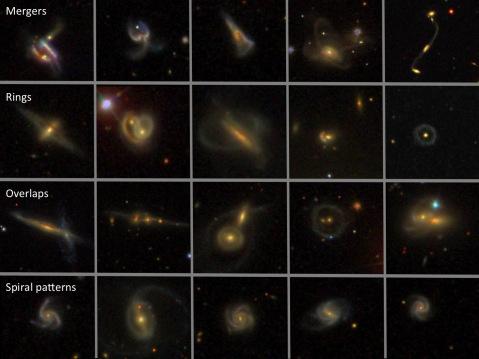
\includegraphics[width=.7\textwidth, height=.4\textheight]{figures/galaxyclass.jpg}
    \caption{Galaxy features laid out in the Galaxy Zoo project}
\end{figure}

\chapter{Literature Review}
\section{ANN and analysing the RMS dispersion}
\hspace*{0.5 in}\cite{Naim/mnras/275.3.567} attempted the first ever automated classification using supervised artificial neural networks. They trained the network based on the morphology of the galaxy images as they appear on the blue survey plates. The network was used to classify images from the Automated Plate Measurement (APM) Equitorial Catalogue of Galaxies while reducing each image to the morphological features such as number of spiral arms and bulge size. By using this Supervised approach,the RMS dispersion between the ANN type and correct mean type was comparable to the overall RMS dispersion between the experts. 
\section{Implementaion of decision trees}
\hspace*{0.5 in}Decision trees had proven themselves to be quite useful in automated classification techniques in a number of astronomical domains. \cite{Owens/mnras/281.1.153} employed oblique decision trees for the morphological classification using the data from \cite{Storrie1992}.They also indicated that the data could be classified into lesser, but well defined categories. Galaxies could now be confidently classified to larger, overlapping regions, i.e. that multiple decision trees could, in fact, be generated to distinguish easily between different regions along the continuum of classifications.This essentially meant that, while the non-neighbour classes could be easily separated, the neighbouring classes could not. While trees grown to distinguish E-type galaxies from Sa+Sb-types were accurate but those grown to distinguish E-types from S0-types would be very inaccurate (Refer Fig. \ref{HubbleTuningFork}).
\section{Naive Bayes and Decision Tree induction algorithm}
\hspace*{0.5 in}\cite{Bazell_2001} showed a comparison of three algorithms for automated galaxy classification. They used a Naive Bayes classifier and a decision-tree induction algorithm with pruning for automated classification of 800 galaxies, proving that an ensemble of classifiers decreases the classification error.The results show that (1) the neural network produced the best individual classifiers (lowest classification error) for the majority of cases, (2) the ensemble approach significantly reduced the classification error for the neural network and the decision-tree classifiers but not for the Naive Bayes classifier, (3) the ensemble approach worked better for decision trees (typical error reduction of 12\%-23\%) than for the neural network (typical error reduction of 7\%-12\%), and (4) the relative improvement when using ensembles decreases as the number of output classes increases. While more extensive comparisons are needed (e.g., a variety of data and classifiers), our work is the first demonstration that the ensemble approach can significantly increase the performance of certain automated classification methods when applied to the domain of morphological galaxy classification.

\begin{table}[t]
\centering
\tiny
\begin{tabular}{p{4cm} l} 
\hline
\hline
 Feature Name & Description\\ 
 \hline
 Peak brightness\dotfill & Maximum brightness level in image\\ 
 $m_{q2q3}$\dotfill & Ratio of fitted slope of $I(r)$ vs $r$ for the second and third quartiles\\
 Ellipticity\dotfill & Ratio of the semimajor to semiminor axis length\\
 Area\dotfill & Number of pixels contained in the object\\
 Max(rI)\dotfill & Maximum value of the plot of $rI(r)$ vs. $r$\\
 Asym\dotfill & Comparision between original galaxy and galaxy rotated $180^{\circ}$\\
 $r_25/r_75$\dotfill & Ratio of radii at which 25\% and 75\% of light is enclosed in a plot of $I(r)$ vs $r$\\
 $R_{Bulge}$\dotfill & Radius where $I(r)$ falls to 90\% of peak value\\
 $C_3, C_6$\dotfill & Concentration indices for the annuli 3 and 6\\
 Isophotal displacement\dotfill & Maximum displacement of the centres of five isophotal levels\\
 Isophotal filling factor\dotfill & Area of an isophotal level relative to the area of the enclosing ellipse\\
 $P_{max}$\dotfill & Maximum value of the normalized co-occurence matrix, $c_{ij}$\\
 Entropy\dotfill & $-\sum_{i,j}{c_{ij} log{(c_{ij})}}$\\
 \hline
\end{tabular}
    \caption{Description of features used in morphological classification}
    \label{features_morphological}
\end{table} 

\vspace{3\baselineskip}
\section{Neural networks with Locally weighted regression}
\hspace*{0.5 in}\cite{De_La_Calleja2004} used a neural network along with a locally weighted regression method, and implemented a homogeneous ensembles of classifiers. It was found that accuracy dropped from 95.11\% to 92.58\% while classifying galaxies into two classes (E and S) to three classes (E, S, Irr). Further increase in classes caused the accuracy to drop further i.e. accuracy of 56.33\% for a five-case classification which further reduced to 48.50\% for a seven-case classification.

\hspace*{0.5 in}\cite{Banerji_2010} employed Artifical Neural Network to classify  galaxies into three classes ie.spirals,early types,point sources. A combination of the profile fitting and adaptive weighted fitting parameters resulted in better than 90\% accuracy, it was observed that the input parameters are more decisive in achieving greater accuracy than the completeness of magnitude of the training set. \cite{Gauci2010} applied and compared Decision tree algorithms using CART and C4.5, Random Forests and fuzzy logic algorithms. While promising results were achieved in all the employed algorithms, Random Forests gave the highest accuracy.

\section{Linear Discriminant Analysis Technique}
\hspace*{0.5 in}\cite{Ferrari_2015} presented an extented morphometric system which classified galaxies automatically based on the CASGM coefficients (Concentration, Asymmetry, Smoothness) along with some new parameters such as Entropy and spirality. Using the data from the Galaxy zoo project, spiral and elliptical galaxies were used for training, a Linear Discriminant Analysis (LDA) technique was employed to classify the galaxy samples. The cross validation showed that the accuracy achieved was about 90\%. The approach was not simple visual inspection but rather based the scheme on physical characteristics of the galaxies (e.g. age weighted using luminosity or mass) and it was observed that the results matched closely with the visual classification. 
\section{Feature extraction and Convolutional Networks}
\hspace*{0.5 in}\cite{Lecun2015} showed how the performance of classification depends on feature engineering. The feature engineering and feature extraction played an important role in classification models as further models exploited the elemental features of a galaxy image and used advanced algorithms to classify them. Deep learning models consists of multiple non-linear layers which learn data representations and automatically extract features from the raw data that is fed into it \citep{Bengio2013,Lecun2015}.\\
\hspace*{0.5 in}After a series of non-linear transformations, the higher levels have abstract representations of data and these can essentially be used for discrimination and classification purposes. Thus, deep convolutional neural networks (CNNs) have become a particularly dominant approach for image classification and feature extraction. The tremendous datasets such as the Galaxy Zoo which are well equipped with the predefined data representations allow faster and efficient implementation of these CNNs, with many works yielding excellent results.\\
\hspace*{0.5 in}\cite{Mairal2014} proposed to train convolutional neural networks to approximate kernel feature maps, which allow the desired invariance properties to be encoded in the choice of kernel, and subsequently be learnt.\\
\hspace*{0.5 in}The first ever attempt at classifying galaxies using a convolutional architecture was made by \cite{Dieleman2015} by implementing a 7-layer model. He classified the galaxies based on their morphological features by translation of the images and exploiting the rotational invariance of galaxies.Then, \cite{Huertas-Company_2011} used the Dieleman model to classify high redshift galaxies in the 5 Cosmic Assembly Near-infrared Deep Extragalactic Legacy Survey (CANDELS). \cite{Kim&Brunner} presented a star–galaxy classification framework that uses deep ConvNets directly on the reduced, calibrated pixel values. Using data from the Sloan Digital Sky Survey and the Canada–France–Hawaii Telescope Lensing Survey, they demonstrated that ConvNets are able to produce accurate and well-calibrated probabilistic classifications that are competitive with conventional machine learning techniques.\\
\hspace*{0.5 in}Later, \cite{dai2018galaxy} implemented a combination of the Dieleman model along with the residual network (ResNets) proposed by \cite{He_2016} to classify the galaxies into 5 classes and achieved an accuracy of 95.2083\% on the testing set.
\chapter{Problem Definition}
\hspace*{0.5 in}Through numerous methods and approaches, galaxies were being classified into their respective classes rapidly. The problem of efficiency still remained as the importance of galaxy classes kept increasing. The methods that achieved an excellent accuracy for binary classifications mainly spiral and elliptical were particularly failing to achieve the same if the number of classes were increased. Furthermore, the classes that formed were refined over the years as more and more galaxies were discovered. It was observed that networks with over 90\% testing accuracy with binary classifications had their accuracy reduced by almost half when introduced with a new class (e.g. irregular). This was making it harder to develop a method that was efficient. On the other hand, the data that was provided by the surveys kept on increasing. Thus, a new approach was necessary for galaxy classification with more refined classes and maximum efficiency.
\chapter{Solution}
\section{Dieleman Model}
\subsection{Methodology}
\hspace*{0.5 in}Dieleman was the first person to propose a deep convolution model for galaxy morphology classification. He observed the drawback of the restricted connectivity patterns in convolutional networks. These result in reduced parameters required for modelling large images. But by exploiting the translational symmetry of the images, it could function to increase them. Furthermore, other invariances exist that could essentially improve the amount of parameters used for modelling a better network. Rotational invariance could be one of these as rotating a galaxy would have no effect on the morphology of the galaxy. Thus, exploiting the rotational invariance would provide better results in generalizing the classifications. Though, it was easier to use the translational symmetry for a convolutional network the same was not the case to implement a rotational invariance. Application of the same rotation filter would have to have different instances of translation applied. Rotating the image by any other angle which is not a multiple of $90^{\circ}$ would result in missing pixels which would need interpolation to fill. These complications made exploiting the rotational symmetries much more difficult.\\
\hspace*{0.5 in}The dataset provided by the Galaxy Zoo project had been observed to have some images that were vertically and horizontally flipped as an experiment with the crowdsourced classification. \citet{Land_et_all_2008} showed showed that the raw votes had an excess of 2.5\% for S-wise (anticlockwise) spiral galaxies over Z-wise (clockwise) galaxies. Since this effect was seen in both the raw and mirrored images, it was interpreted as a bias due to preferences in the human brain, rather than as a true excess in the number of apparent S-wise spirals in the Universe. The Galaxy Zoo 2 probabilities do not contain any structures related to handedness or rotation-variant quantities, and no rotational or translational biases have yet been discovered in the data. If such biases do exist, however, this would presumably reduce the predictive power of the model since the assumption of rotational
invariance to the output probabilities would no longer apply.\\

\begin{figure}[h]
    \centering
    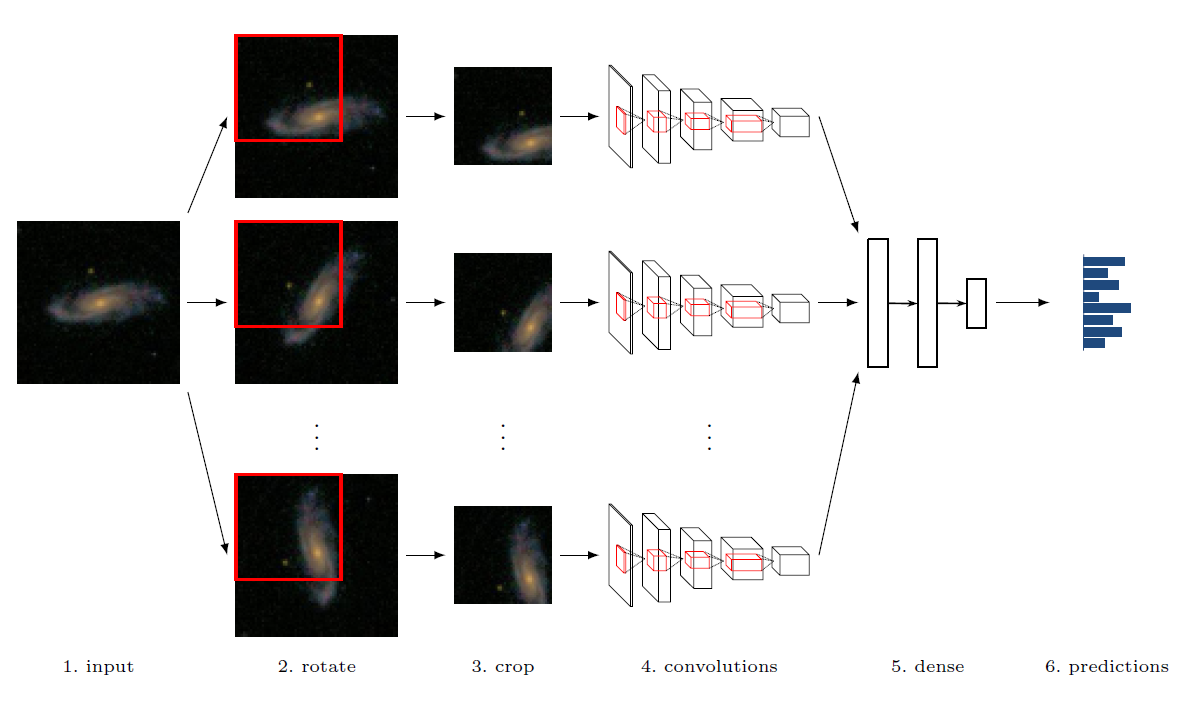
\includegraphics[width=\textwidth, height=.4\textheight]{figures/Dieleman.png}
    \caption{Schematic overview of Dieleman approach}
    \label{DielemanImg}
\end{figure}
\vspace{\baselineskip}
\hspace*{0.5 in}Deep neural networks have a large number of lernable parameters as opposed to the limited training data. As a result, there is a high risk of overfitting, i.e. a network will memorize the training example because it has enough capacity. To tackle this, \citet{Dieleman2015} used many techniques:
\vspace{\baselineskip}
\begin{itemize}
    \item \textbf{data augmentation} : extending the training set by randomly perturbing images in a way that leaves their associated answer probabilities unchanged;
    \item \textbf{regularization} : penalizing model complexity through use of dropout;
    \item \textbf{parameter sharing} : reducing the number of model parameters by exploiting translational and rotational symmetry in the input images;
    \item \textbf{model averaging} : averaging the predictions of several models.
\end{itemize}

\begin{figure}[h]
    \centering
    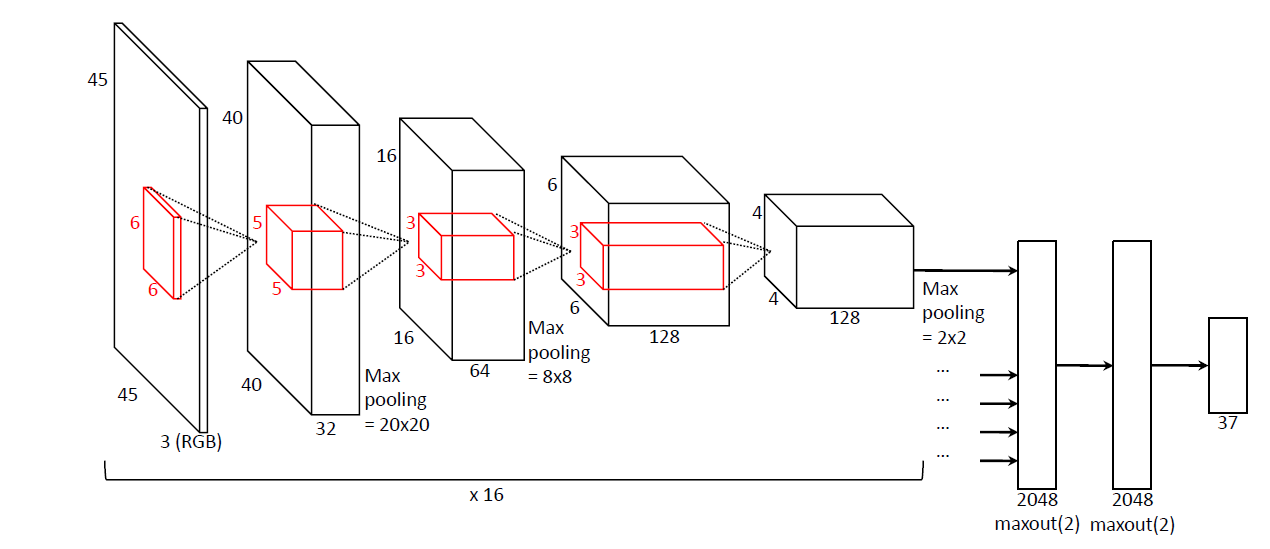
\includegraphics[width=\textwidth, height=.4\textheight]{figures/Dieleman_model.png}
    \caption{Schematic overview of the model architecture}
    \label{DielemanModel}
\end{figure}
\subsection{Results}
\hspace*{0.5 in}The dataset used was from the Galaxy Zoo 2 which was a collection of answers from the decision tree in table \ref{GZ2_DecisionTree}).\\
\hspace*{0.5 in} Dieleman achieved an RMSE score of 0.7671 for the best performing network and later, he averaged the results over 17 networks to get an RMSE score of 0.7467. The results for precision and recall pf each question in the GZ2 tree (refer table \ref{GZ2_DecisionTree}) have been summarized in the table \ref{DielemanResults}.
\begin{table}[H]
\begin{adjustbox}{width=0.39\textheight,center}
\begin{tabular}{c p{5 cm} l r} 
\hline
 Task & Question & Responses & Next\\
\hline
\hline
\multirow{3}{*}{01} & \multirow{3}{*} {\thead[l]{Is the galaxy simply smooth\\ and rounded, with no sign of\\a disk?}} & smooth & 07\\
& & features or disk & 02\\
&  & star or artifact & \textbf{end}\\
\hline
\multirow{2}{*}{02} & \multirow{2}{*} {\thead[l]{Could this be a disk viewed\\ edge-on?}} & yes & 09\\
& & no & 03\\
\hline
\multirow{3}{*}{03} & \multirow{3}{*} {\thead[l]{Is there a sign of a bar\\feature through the centre\\of the galaxy?}} & yes & 04\\
& & no & 04\\
\vspace{1\baselineskip}\\
\hline
\multirow{2}{*}{04} & \multirow{2}{*} {\thead[l]{Is there any sign of a\\spiral arm pattern?}} & yes & 10\\
& & no & 05\\
\hline
\multirow{4}{*}{05} & \multirow{3}{*} {\thead[l]{How prominent is the\\central bulge, compared\\with the rest of the galaxy?}} & no bulge & 06\\
& & just noticible & 06\\
& & obvious & 06\\
& & dominant & 06\\
\hline
\multirow{2}{*}{}06 & \multirow{1}{*} {\thead[l]{Is there anything odd?}} & yes & 08\\
& & no & \textbf{end}\\
\hline
\multirow{3}{*}{}07 & \multirow{1}{*} {\thead[l]{How rounded is it?}} & completely round & 06\\
& & in between & 06\\
&  & cigar-shaped & 06\\
\hline
\multirow{7}{*}{}08 & \multirow{3}{*} {\thead[l]{Is the odd feature a ring,\\or is the galaxy distributed\\or irregular?}} & ring & \textbf{end}\\
& & lens or arc & \textbf{end}\\
& & distributed & \textbf{end}\\
& & irregular & \textbf{end}\\
& & other & \textbf{end}\\
& & merger & \textbf{end}\\
& & dust lane & \textbf{end}\\
\hline
\multirow{3}{*}{09} & \multirow{3}{*} {\thead[l]{Does the galaxy have a\\bulge at its centre? If\\so, what shape?}} & rounded & 06\\
& & boxy & 06\\
&  & no bulge & 06\\
\hline
\multirow{3}{*}{}10 & \multirow{2}{*} {\thead[l]{How tightly wound do the\\spiral arms appear?}} & tight & 11\\
& & medium & 11\\
&  & loose & 11\\
\hline
\multirow{6}{*}{}11 & \multirow{2}{*} {\thead[l]{How many spiral arms\\are there?}} & 1 & 05\\
& & 2 & 05\\
& & 3 & 05\\
& & 4 & 05\\
& & more than four & 05\\
& & can't tell & 05\\
\hline
\end{tabular}
\end{adjustbox}
    \caption{The GZ2 decision tree, comprising of 11 tasks and 37 responses.}
    \label{GZ2_DecisionTree}
\end{table} 

\begin{table}[H]
\begin{adjustbox}{width=0.37\textheight,center}
\begin{tabular}{c p{5 cm} c c c} 
\hline
  & & \textbf{precision} & \textbf{recall} & \textbf{\#example}\\
\hline
\multicolumn{4}{l}{\thead[l]{Q1: smoothness}} & 6144\\
\hline
A1.1 & smooth & 0.8459 & 0.8841 & 2700\\
A1.2 & features or disk & 0.9051 & 0.8742 & 3435\\
A1.3 & star or artifact & 1.0000 & 0.4444 & 9\\
\hline
\multicolumn{4}{l}{\thead[l]{Q2: edge-on}} & 3362\\
\hline
A2.1 & yes & 0.9065 & 0.8885 & 655\\
A2.2 & no & 0.9732 & 0.9778 & 2707\\
\hline
\multicolumn{4}{l}{\thead[l]{Q3: bar}} & 2449\\
\hline
A3.1 & yes & 0.7725 & 0.7101 & 483\\
A3.2 & no & 0.9302 & 0.9486 & 1966\\
\hline
\multicolumn{4}{l}{\thead[l]{Q4: spiral}} & 2449\\
\hline
A4.1 & yes & 0.8715 & 0.8270 & 1451\\
A4.2 & no & 0.7659 & 0.8226 & 998\\
\hline
\multicolumn{4}{l}{\thead[l]{Q5: bulge}} & 2449\\
\hline
A5.1 & no bulge & 0.6697 & 0.5000 & 146\\
A5.2 & just noticeable & 0.7828 & 0.8475 & 1174\\
A5.3 & obvious & 0.8292 & 0.8049 & 1092\\
A5.4 & dominant & 0.4444 & 0.1081 & 37\\
\hline
\multicolumn{4}{l}{\thead[l]{Q6: anything odd}} & 6144\\
\hline
A6.1 & yes & 0.8438 & 0.7500 & 828\\
A6.2 & no & 0.9617 & 0.9784 & 5316\\
\hline
\multicolumn{4}{l}{\thead[l]{Q7: roundedness}} & 2619\\
\hline
A7.1 & completely round & 0.9228 & 0.9282 & 1197\\
A7.2 & in between & 0.9128 & 0.9171 & 1279\\
A7.3 & cigar-shaped & 0.9000 & 0.8182 & 143\\
\hline
\multicolumn{4}{l}{\thead[l]{Q8: odd feature}} & 824\\
\hline
A8.1 & ring & 0.9097 & 0.9161 & 143\\
A8.2 & lens or arc & ? & 0.0000 & 2\\
A8.3 & disturbed & 0.8000 & 0.4138 & 29\\
A8.4 & irregular & 0.8579 & 0.8674 & 181\\
A8.5 & other & 0.6842 & 0.6810 & 210\\
A8.6 & merger & 0.7398 & 0.7773 & 256\\
A8.7 & dust lane & 0.5000 & 0.6667 & 3\\
\hline
\multicolumn{4}{l}{\thead[l]{Q9: bulge shape}} & 493\\
\hline
A9.1 & rounded & 0.9143 & 0.9412 & 340\\
A9.2 & boxy & ? & 0.0000 & 8\\
A9.3 & no bulge & 0.8601 & 0.8483 & 145\\
\hline
\multicolumn{4}{l}{\thead[l]{Q10: arm tightness}} & 1049\\
\hline
A10.1 & tight & 0.7500 & 0.7350 & 449\\
A10.2 & medium & 0.6619 & 0.7112 & 457\\
A10.3 & loose & 0.7373 & 0.6084 & 143\\
\hline
\multicolumn{4}{l}{\thead[l]{Q11: no. of arms}} & 1049\\
\hline
A11.1 & 1 & 1.0000 & 0.2037 & 54\\
A11.2 & 2 & 0.8201 & 0.8691 & 619\\
A11.3 & 3 & 0.4912 & 0.3182 & 88\\
A11.4 & 4 & ? & 0.0000 & 21\\
A11.5 & more than 4 & 0.4000 & 0.4000 & 20\\
A11.6 & can't tell & 0.5967 & 0.7368 & 247\\
\hline
\end{tabular}
\end{adjustbox}
    \caption{Precision and recall scores for each answer}
    \label{DielemanResults}
\end{table}


\section{Very deep convolutional neural networks}
\subsection{Residual Networks}
\hspace*{0.5 in}After the celebrated victory of AlexNet \citep{AlexNet} at the LSVRC2012 classification contest, deep Residual Network \citep{He_2016} was arguably the most groundbreaking work in the computer vision/deep learning community in the last few years. ResNet makes it possible to train up to hundreds or even thousands of layers and still achieves compelling performance.\\
\hspace*{0.5 in}According to the universal approximation theorem, given enough capacity, we know that a feedforward network with a single layer is sufficient to represent any function. However, the layer might be massive and the network is prone to overfitting the data. Therefore, there is a common trend in the research community that our network architecture needs to go deeper. Since AlexNet, the state-of-the-art CNN architecture is going deeper and deeper. While AlexNet had only 5 convolutional layers, the VGG network \citep{VGG2014} and GoogleNet (also codenamed InceptionV1) \citep{Inception2014} had 19 and 22 layers respectively.\\
\hspace*{0.5 in}However, increasing network depth does not work by simply stacking layers together. Deep networks are hard to train because of the notorious vanishing gradient problem — as the gradient is back-propagated to earlier layers, repeated multiplication may make the gradient infinitively small. As a result, as the network goes deeper, its performance gets saturated or even starts degrading rapidly.\\
\hspace*{0.5 in}Before ResNet, there had been several ways to deal the vanishing gradient issue, for instance, \citet{Inception2014} adds an auxiliary loss in a middle layer as extra supervision, but none seemed to really tackle the problem once and for all.\\
\begin{figure}[H]
    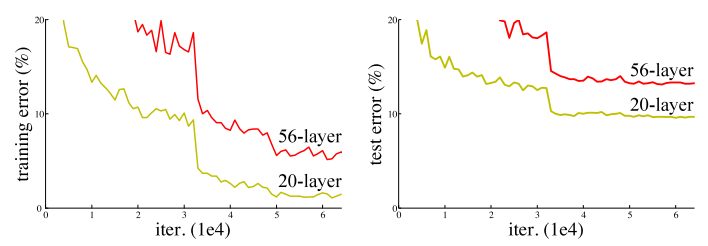
\includegraphics[width=\textwidth]{figures/DeepLayers.png}
    \caption{Performance after increasing no. of layers over training (left) and testing (right)}
    \label{depth_CNN}
\end{figure}

\hspace*{0.5 in}The core idea of ResNet is introducing a so-called “identity shortcut connection” that skips one or more layers, as shown in the figure \ref{ResidualBlock}.
\begin{figure}[H]
    \centering
    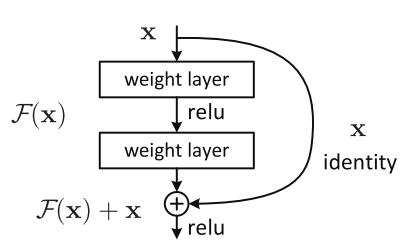
\includegraphics[width=0.5\textwidth]{figures/Residual_block.png}
    \caption{Residual Block with skip connection}
    \label{ResidualBlock}
\end{figure}
\hspace*{0.5 in}\citet{He_2016} argue that stacking layers shouldn’t degrade the network performance, because we could simply stack identity mappings (layer that doesn’t do anything) upon the current network, and the resulting architecture would perform the same. This indicates that the deeper model should not produce a training error higher than its shallower counterparts. They hypothesize that letting the stacked layers fit a residual mapping is easier than letting them directly fit the desired underlaying mapping. And the residual block above explicitly allows it to do precisely that. Because of its compelling results, ResNet quickly became one of the most popular architectures in various computer vision tasks.
\begin{figure}[H]
    \centering
    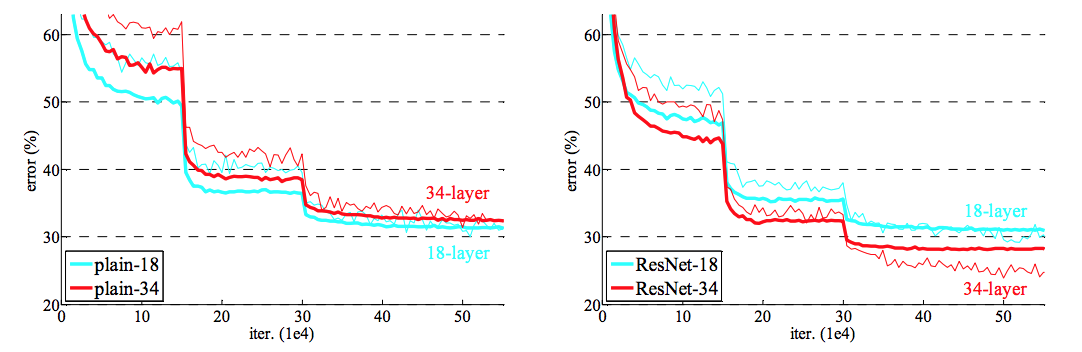
\includegraphics[width=\textwidth]{figures/PlainVsResnet.png}
    \caption{Residual Block with skip connection}
    \label{PlainVsResidual}
\end{figure}
\hspace*{0.5 in}The following table shows how testing error of different depths:
\begin{table}[H]
    \centering
    \begin{tabular}{c | c c}
         & plain & ResNet \\
         \hline
        18 layers & 27.94 & 27.88\\
        34 layers & 28.54 & 25.03\\
    \end{tabular}
    \caption{Testing error over different depths}
    \label{TestPlainVsResNets}
\end{table}
\begin{figure}[H]
    \centering
    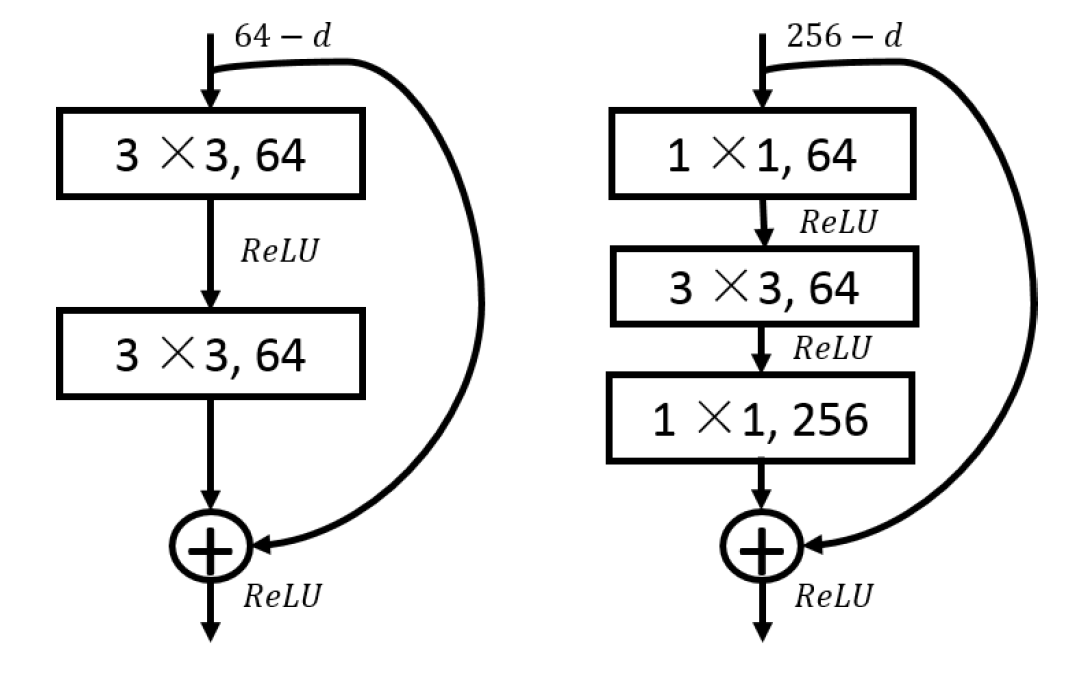
\includegraphics[width=0.4\textwidth]{figures/BottleNeckResnet.png}
    \caption{A deeper residual function F. Left: a building block as in Figure \ref{ResidualBlock} for ResNet-34. Right: a "bottleneck" building block for ResNet-50/101/152/200.}
    \label{BottleNeckBlock}
\end{figure}

\newpage
\subsection{J. M. Dai model}
\subsubsection{Methodology}
\hspace*{0.5 in}\citet{dai2018galaxy} proposed a variant of residual networks combined with the Dieleman approach for galaxy morphology classification. Instead of working on predicting the results in the manner that Dieleman did with 37 classes from the GZ2 dataset, \citet{dai2018galaxy} used the data as a result to classify galaxies into five classes i.e. completely round smooth, in-between smooth (between completely round and cigar-shaped), cigar-shaped smooth, edge-on and spiral. The galaxy images were drawn from The Galaxy Zoo challenge \citep{Willett_2013} which contained 61578 images with probabilities that each galaxy is classified into different morphologies. The morphological classifications vote fractions are modifed version of the weighted vote fractions in the Galaxy Zoo 2 project. The classifications vote fractions have high level of agreement and authority with professional astronomers \citep{Willett_2013}. \citet{dai2018galaxy} cleaned the samples in a way where each sample matched a specific morphological category with its appropriate threshold. The thresholds depended on the number of votes for a classification task considered to be sufficient for that morphology. By this means, they assigned galaxy images to five classes, i.e. completely round smooth, in-between smooth(between completely round and cigar-shaped), cigar-shaped smooth, edge-on and spiral. The 5 classes contain a sample of 8434, 8069, 578, 3903 and 7806 respectively. The dataset reduced to 28790 images after filtering, then
was divided into training set and testing set by a ratio of 9:1. Thus the network was trained over 25911 images and tested over 2879 images.\\
\begin{figure}[H]
    \centering
    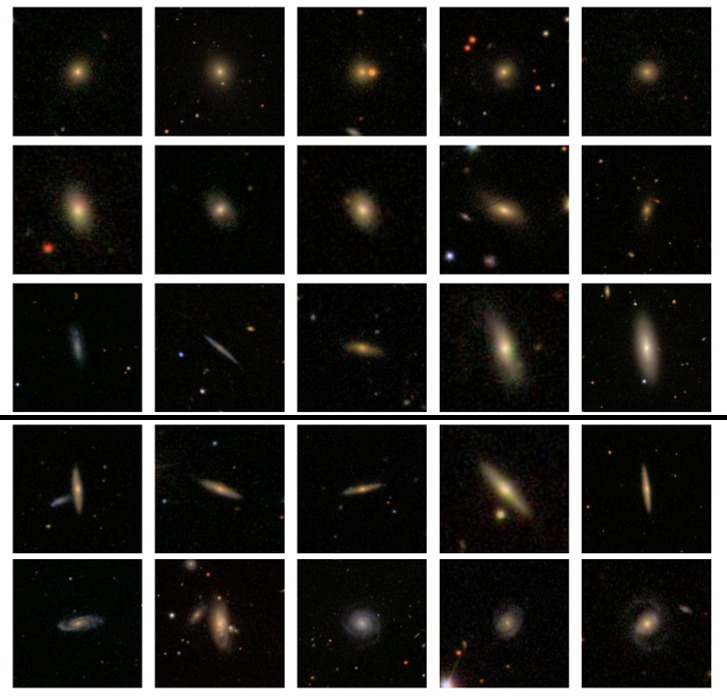
\includegraphics[width=0.5\textwidth]{figures/DaiClasses.jpeg}
    \caption{Example galaxy images from the dataset. Each row represents a class. From top to bottom, their Galaxy Zoo 2 labels are: completely round smooth, in-between smooth, cigar-shaped smooth, edge-on and spiral. Reproduced from \citep{dai2018galaxy}.}
    \label{DaiClasses}
\end{figure}
\hspace*{0.5 in}In order to avoid overfitting, data augmentation is one of the common and effective ways to reduce overfitting. Because of limited training data, data augmentation can enlarge the number of training images. \citep{dai2018galaxy} used five different forms
of data augmentation. Scale jittering is the first form of data augmentation.
In training time, they crop the images to a range scale S =[170; 240] , which is called multi-scale training images because of the S random value. Since different images can be
cropped to different sizes and even the same images also can be cropped to different sizes at different iterations, it is beneficial to take this into account during training. This can be
seen as training set augmentation by scale jittering. Random cropping is carried out from 80 x 80 x 3 pixels to 64 x 64 x 3 pixels, which increases the size of training set by a factor of 256. Rotating training images with $0^{\circ}$; $90^{\circ}$; $180^{\circ}$; $270^{\circ}$ can enlarge the size of training set by a factor of 4. A horizontal flipping is a doubling of training images.\\
\begin{figure}[H]
    \centering
    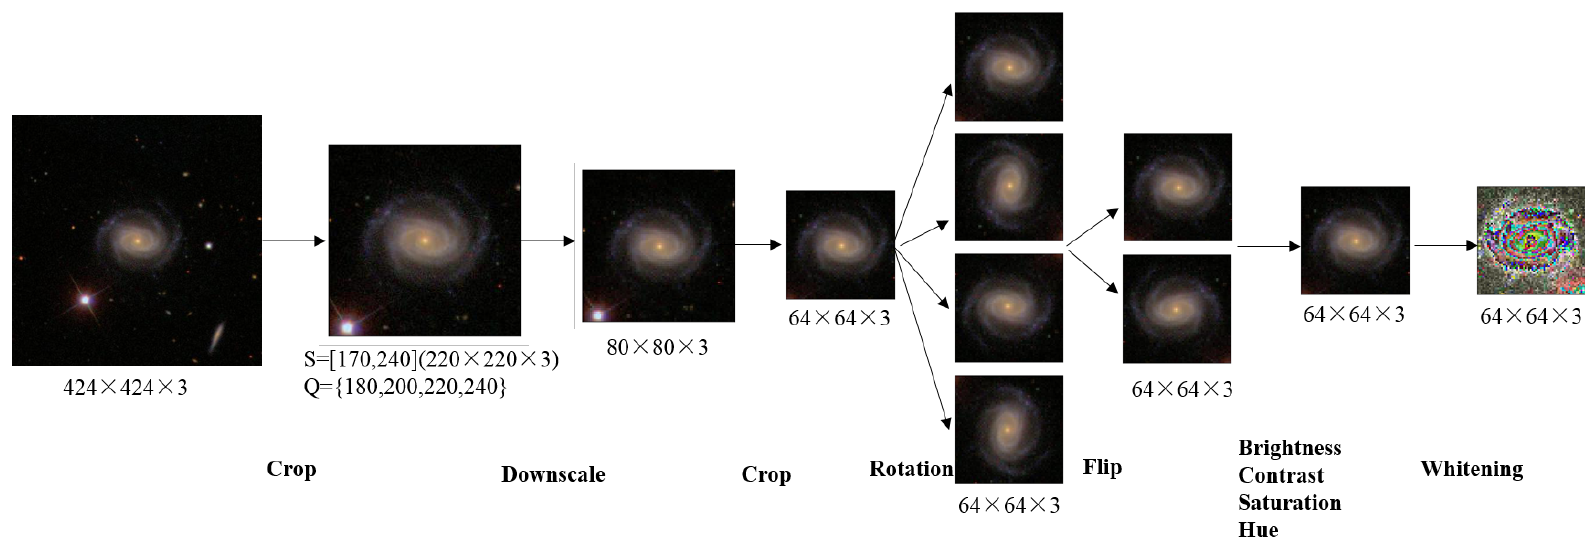
\includegraphics[width=\textwidth]{figures/Preprocessing.png}
    \caption{Preprocessing procedure. The original image firstly is center cropped to a range scale S = [170; 240] in training set (Q ={180, 200, 220, 240} in testing set), for example, the spiral galaxy (GalaxyID:237308) is cropped to 220 x 220 x 3 pixels, then resized to 80 x 80 x 3 pixels, randomly cropped to 64 x 64 x 3 pixels, randomly rotated $0^{\circ}$; $90^{\circ}$; $180^{\circ}$; $270^{\circ}$, and randomly horizontally flipped. After optical distorting and image whitening, it (64 x 64 x 3 pixels) becomes the input of networks.}
    \label{preprocessing_dai}
\end{figure}
\hspace*{0.5 in}The model that \citep{dai2018galaxy} came up with was a variant of ResNets V2. They built a network that was specifically designed for galaxies and tried to decrease depth and widen the residual networks. They adopted a full pre-activation residual units and a "bottleneck" building block( Figure \ref{BottleNeckBlock}, right) presented in \citep{He2016a} is used, namely, a combination of 1 x 1; 3 x 3; 1 x 1 convolutions. The full pre-activation includes standard "BN-ReLU-Conv". In addition to these, we add a dropout after 3 x 3 convolution whereas ResNet V2 \citep{He2016a} did not use dropout to prevent coadaptation and overfitting. The residual unit is defined as:

$x_{l+1} = x_l + W_3\sigma(W_2\sigma(W_1\sigma(x_l))).$\\
\hspace*{0.5 in}Here, $x_l$ and $x_{l+1}$ are input and output of the l-th unit, $\sigma$ denotes BN and ReLU, $W_1,W_2,W_3$ represent 3 convolutional kernels, dropout is placed after the $W_2$ operation and the biases are omitted for simplifying notations.

\begin{figure}[H]
    \centering
    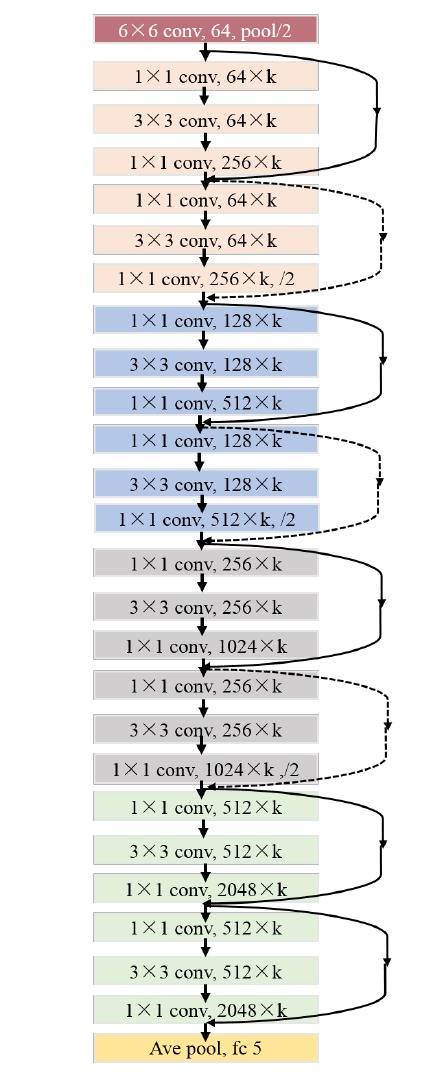
\includegraphics[height=0.95\textheight]{figures/DaiNetwork.jpeg}
    \caption{Network architecture for Galaxy by \citep{dai2018galaxy} where k is the widening factor.}
    \label{dainetwork}
\end{figure}
\subsubsection{Results}
\hspace*{0.5 in}The 5 classes, i.e.  completely round smooth, in-between smooth(betweencompletely  round  and  cigar-shaped),  cigar-shaped  smooth,  edge-on  and  spiral, are labelled starting from 0 through 5. The results obtained by the network are shown below.
\begin{table}[H]
    \centering
    \begin{tabular}{c c c c}
    \hline
    \hline
        class & Precision & Recall & F1\\
    \hline
        0 & 0.9611 & 0.9634 & 0.9622\\
        1 & 0.9561 & 0.9431 & 0.9495\\
        2 & 0.7234 & 0.5862 & 0.6476\\
        3 & 0.9412 & 0.9485 & 0.9448\\
        4 & 0.9573 & 0.9782 & 0.9677\\
        Average & 0.9512 & 0.9521 & 0.9515\\
    \hline
    \end{tabular}
    \caption{Precision, Recall and F1 for each class on testing set.}
    \label{ResultaDai}
\end{table}
\begin{table}[H]
    \centering
    \begin{tabular}{c|c c c c c}
        \hline
        & 0 & 1 & 2 & 3 & 4\\
        \hline
        0 & \textbf{815} & 21 & 0 & 0 & 10\\
        1 & 29 & \textbf{762} & 0 & 0 & 17\\
        2 & 0 & 4 & \textbf{34} & 18 & 2\\
        3 & 0 & 3 & 12 & \textbf{368} & 5\\
        4 & 4 & 7 & 1 & 5 & \textbf{763}\\
        \hline
    \end{tabular}
    \caption{Confusion matrix for each class on testing set. Column represents true label and row represents prediction label.}
    \label{confusionmatrix}
\end{table}
\chapter{Conclusion}
\hspace*{0.5 in}The problem of galaxy morphology and their classification has been of major concern for the past century. Modern technology has facilitated growth of multiple techniques which use large computation power. Neural networks have been applied as a classification technology owing to the sheer volume of data. Research conducted so far has shown that accurate classification of galaxies can be made between two classes, namely spiral and elliptical. It has also been observed that increasing the number of classes results in a decreasing accuracy and less precision. \citet{dai2018galaxy} have attempted to solve the problem by proposing a deep convolution network which combines the model proposed by \citet{Dieleman2015} and the ResNets proposed by \citet{He_2016}. The data used from The Galaxy Zoo project \citep{Willett_2013} is used for training. The model has been able to predict the classes with an overall accuracy of 95.2083\% over the testing set. The solution is able to use the data from galaxy images and predict the morphology of the galaxy. The resulting prediction allows the classification of galaxy images into one of the five classes proposed in \citep{dai2018galaxy}. The results have been far better than all the previous approaches to the problem and seems have formed a promising groundwork for future studies. However, even though the model provides extremely high accuracy, its still expected that the model accuracy shall plummet as the number of classes increases. Further studies can result in even better models that may be then applied to large scale galaxy classification and cluster surveys such as the Large Synoptic Survey Telescope (LSST).

\renewcommand\bibname{References}
\bibliographystyle{apalike}
\bibliography{References}
\end{document}